\documentclass[12pt]{article}

\usepackage[spanish]{babel}
\usepackage[utf8x]{inputenc}
\usepackage{amsmath}

\usepackage{hyperref}
\usepackage{url}
\usepackage{gensymb}
\usepackage[dvipsnames]{xcolor}

\usepackage{parskip}
\usepackage{fancyhdr}
\usepackage{multicol}
\usepackage{vmargin}
\usepackage{setspace}
\usepackage{geometry}

\usepackage{float}
\usepackage{array}
\usepackage{graphicx}
\graphicspath{{images/}}
\usepackage{wrapfig}
\usepackage{caption}
\usepackage{subcaption}

\setmarginsrb{2 cm}{1 cm}{2 cm}{1.5 cm}{1 cm}{1 cm}{1 cm}{1 cm}

\title{Calibración de Termopar}
\author{Martín Alejandro Paredes Sosa}		

\makeatletter
\let\thetitle\@title
\let\theauthor\@author
\let\thedate\@date										
\makeatother

\pagestyle{fancy}
\fancyhf{}
\rhead{Lic.. Física}
\lhead{Informe 3B: \thetitle}
\cfoot{\thepage}

\begin{document}
%%%%%%%%%%%%%%%%%%%%%%%%%%%%%%%%%%%%%%%%%%%%%%%%%%%%%%%%%%%%%%%%%%%%%%%%%%%%%%%%%%%%%%%%
%\begin{titlepage}
%	\centering
%    \vspace*{0.5 cm}
%    
\includegraphics[scale = 0.5]{logo}\\[0.5 cm]	% University Logo
%    \textsc{\LARGE Universidad de Sonora}\\[1 cm]	% University Name
%	\textsc{\Large División de Ciencias Exactas y Naturales}\\[1 cm]		%		% Course Code
%	\textsc{\large Termodinámica Clásica}\\[0.5 cm]				% Course Name
%	\rule{\linewidth}{0.2 mm} \\[0.4 cm]
\begin{center}
{ \large \bfseries \thetitle}\\
\end{center}
%{ \large \bfseries \thetitle}\\
%	\rule{\linewidth}{0.2 mm} \\[1.25 cm]
%    \textsc{\Large Equipo \#2} \\[1.25 cm]
%\thetitle\\	
	\begin{minipage}{\textwidth}
		\begin{center} 
			%\textsc{\Large Integrantes:} \large \\
			\theauthor 
			\end{center}
	\end{minipage}\\[0.2 cm]
%	\vfill
	
%\end{titlepage}
%===================================================================================================
%\pagebreak
%\tableofcontents
%\pagebreak
%===================================================================================================
\begin{abstract}
	Esta practica consistió en tomar un termopar tipo K, y calibrarlo mediante el uso de agua en coexistencia con hielo y con  una mezcla de agua y etilenglicol colocado en un baño recirculador como puntos fijos.
\end{abstract}
\vspace{-1cm}
%===================================================================================================
\section{Introducción}
En está práctica se tomó un termopar tipo K  con el obejetivo de calibrarlo. Para esto se hizo uso de dos puntos fijos. En nuestro caso estos puntos son el punto de fusión normal del agua y el del baño recirculador con la mezcla de agua y etilenglicol que se encontraba a 40 °C.

Un termopar es un a sensor para medir temperatura. Este consiste en dos metales diferentes unidos. Cuando la unión de los dos metales se calienta o enfría se produce un voltaje que se puede correlacionar con la temperatura. El tipo K suelen medir en rango de -200°C a 1250°C con un errores limtes estandar del 2.2°C o 0.75\%. Los metales del que esta compuestos son el cromel (aleación de cromo y nickel) y alumel (aleación de aluminio y aluminio\cite{termopar}.

%===================================================================================================
\section{Desarrollo Experimental}
En este experimento, primeramente se tiene un recipiente con agua y hielo. Se colocó un termometro para obtener un valor aproximado de la temperatura del agua con hielo. En un baño recirculador se tenia una mezcla de agua y etilenglicol a la cual se ajusto a una temperatura de 40°C.
\begin{figure}[H]
\centering
\includegraphics[scale=0.35]{termopar.png}
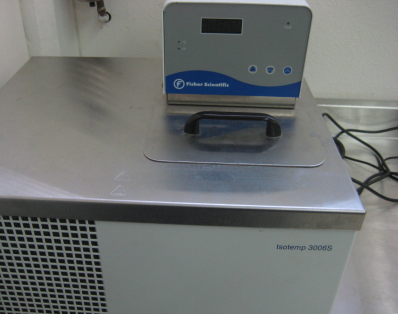
\includegraphics[scale=0.35]{mezcla.png}
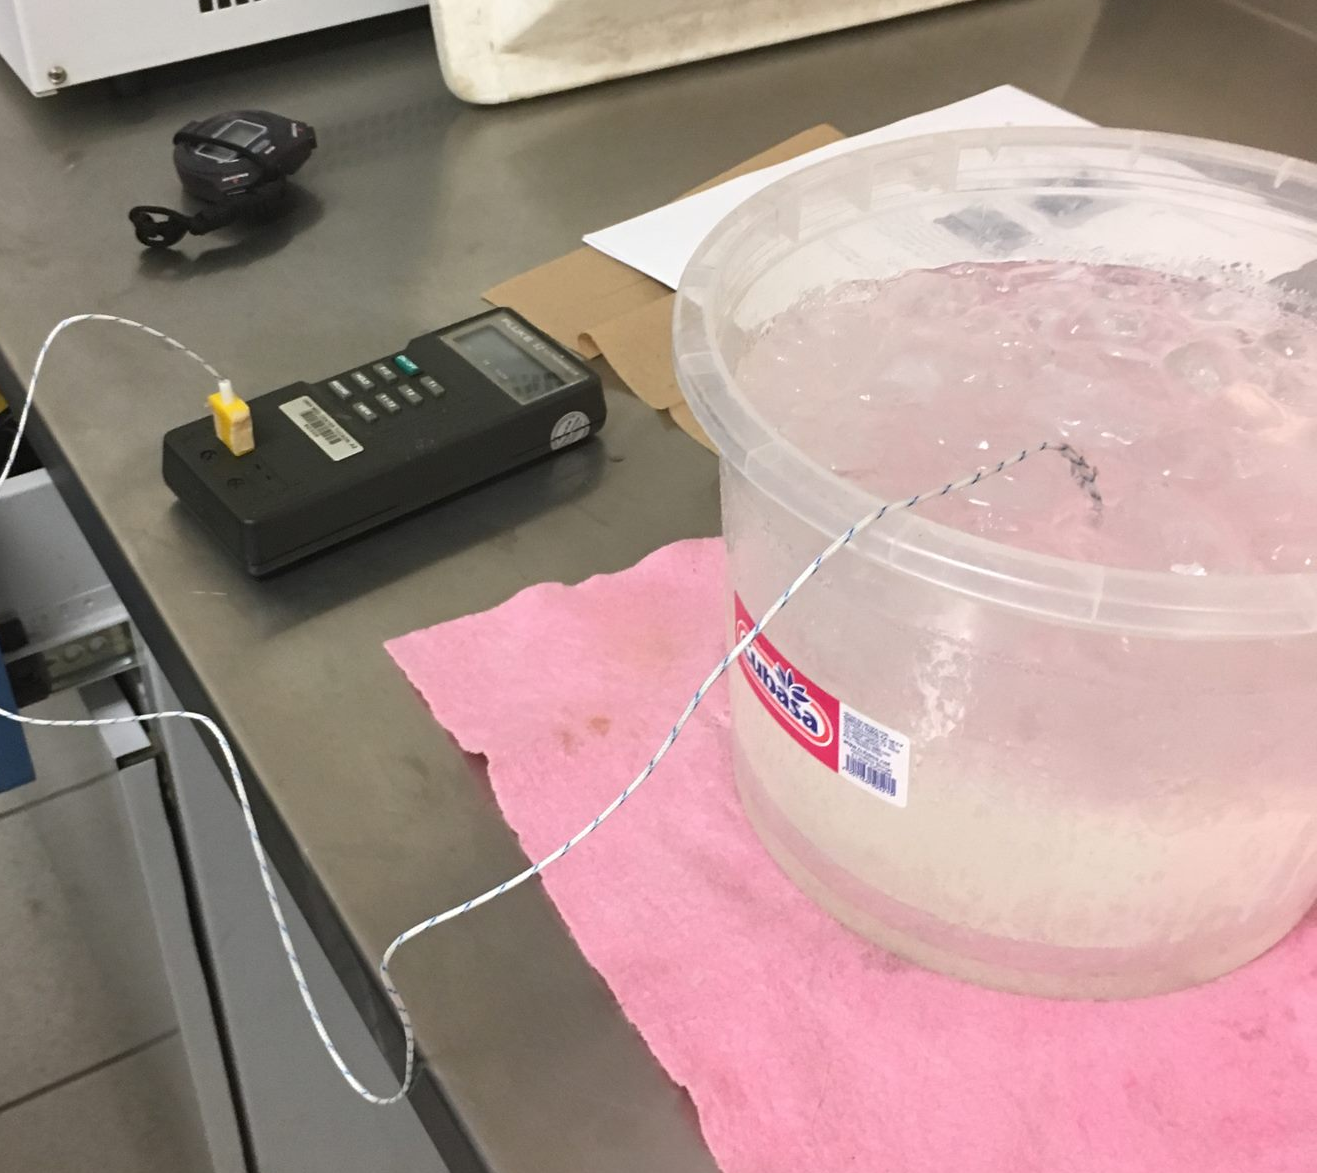
\includegraphics[scale=0.10]{arr.png}
\caption{Arreglo Experimental}
\end{figure}

\hspace*{0.5cm}Se tomo el termopar  tipo K de la marca Fluke. Mide en el intervalo de -200°C a 1250°C con un error limite estándar de 2.2°C. Se puso en contacto térmico el termopar con la mezcla de agua y etilenglicol se ajustó el tornillo para ajustar el valor de la temperatura que mostraba en pantalla el termopar hasta que marcara los 40°C que corresponde al valor de la temperatura a la que se encontraba la mezcla.

\hspace*{0.5cm}Luego se puso en térmico el termopar con la mezcla de agua y hielo el termopar y se observo que el valor que mostraba y se ajusto nuevamente. Se repitio varias veces hasta que se logro realizar una buena calibración.

\pagebreak

%===================================================================================================
\section{Resultados}
En el primer contacto el termopar marco 37.1°C, sin realizar ninguna calibración.

En la siguiente tabla se muestran la temperaturas que marco el termopar con la misma calibración en los sistemas.

\begin{table}[H]
\centering
\begin{tabular}{|c|c|c|}
\hline
Calibración &  Agua y etilenglicol &  Agua con hielo    \\ \hline
   1      &    40°C  $\pm$2.2°C  &   2.3°C $\pm$2.2°C   \\ \hline
   2      &    40°C  $\pm$2.2°C  &   2.1°C $\pm$2.2°C   \\ \hline
   3      &    40°C  $\pm$2.2°C  &   1.8°C $\pm$2.2°C   \\ \hline
   4      &   38.2°C $\pm$2.2°C  &     0°C $\pm$2.2°C   \\ \hline
   5      &    40°C  $\pm$2.2°C  &   1.8°C $\pm$2.2°C   \\ \hline   
\end{tabular}
\caption{Medición de temperatura}
\end{table}
En la cuarta calibración se calibro en el agua con hielo y luego se midió en el agua con etilenglicol.

%===================================================================================================
\section{Discusión}
Lo que se esperaba es que las temperaturas que se mostraran fueran de 40°C en el agua con etilenglicol y 0°C al agua con hielo. Lo que observamos fue que al calibrar con uno, en el segundo sistema existía una diferencia que no se esperaba. Esta se debió a que el agua con hielo, no estaba exactamente a 0°C, ademas de que el termopar no es totalmente exacto.

%===================================================================================================
\section{Conclusiones}
En conclusión, si se pudo calibrar el termopar, dado que a la medida que se obtenía en el baño recirculador era un valor muy cercano, y este aparato es muy eficaz para mantener una temperatura, y el agua con hielo por si solo no mantiene con facilidad la misma temperatura(se mantiene estable).

\pagebreak
%================================================================================================


\begin{thebibliography}{6}
\bibitem{termopar}
OMEGA(s.f.)\textit{Termopar: Tipos y Aplicaciones}. Recuperado de \url{http://es.omega.com/prodinfo/termopares.html}
	
\bibitem{man}
	Fluke Corporation \textit{Fluke51,52}. Recuperado de   \url{http://www.pasco.com}

\bibitem{acu}
Acu\~na, H. (2015). \textit{Manual de Guías de Experiencias en el Laboratorio de Termodinámica Clásica}.

\end{thebibliography}
%================================================================================================

\end{document}